\documentclass[12pt]{article}

\usepackage{sbc-template}
\usepackage{graphicx,url}
\usepackage[utf8]{inputenc}
\usepackage[brazil]{babel}
%\usepackage[latin1]{inputenc} -> Erro
\usepackage{placeins} % para usar o /FloatBarrier
\usepackage{booktabs} %p/ tabelar
\usepackage{algorithm}
\usepackage{algpseudocode}
     
\sloppy

\title{
Relatório técnico para a disciplina de algoritmos em grafos ministrada pelo Prof. Dr. Ademir A. Constantino\\
Algoritmos construtivos e melhorativos para o problema do caixeiro viajante assimétrico
}

\author{Dalvan T. Oliveira\inst{1},  Luiz H. C. M. Marques\inst{1} }


\address{
	Universidade Estadual de Maringá (UEM)\\
	Centro de Tecnologia -- Departamento de Informática\\
	Programa de Pós-Graduação em Ciência da Computação\\
	Maringá -- PR -- Brasil
  \email{dalvan.oliveira@outlook.com, luhenrique06@hotmail.com}
}

\begin{document} 

\maketitle

%\begin{abstract}
%  This meta-paper describes the style to be used in articles and short papers
%  for SBC conferences. For papers in English, you should add just an abstract
%  while for the papers in Portuguese, we also ask for an abstract in
%  Portuguese (``resumo''). In both cases, abstracts should not have more than
%  10 lines and must be in the first page of the paper.
%\end{abstract}
     
\begin{resumo} 
	Neste trabalho foi implementado algoritmos em grafos para resolução do problema
	do caixeiro viajante usando técnicas construtivas e melhorativas.
	É feito uma breve explicação do problema e das técnicas utilizadas.
	A linguagem de programação C foi usada para implementação dos algorítimos e
	foi resolvido as instâncias assimétricas da base de dados TSBLIB.

\end{resumo}


\section{Introdução}
\textbf{pequena introdução sobre o que vamos falar nessa seção...}

\subsection{O problema do caixeiro viajante}
O problema do caixeiro viajante - PCV consiste em visitar
$ v_{1},...,v_{n} $
pontos distintos, partindo de um ponto inicial
$v_{0} = v_{i,}$
para algum
$i=1,...,n,$
de tal forma que não passe mais de uma vez em um mesmo ponto
e além disso, ao término, deve-se voltar ao ponto inicial
$v_{0}.$
Além disso, todos os pontos estão mutualmente conectados e essas
conexões possuem custos.

Pode-se considerar os pontos como clientes.
Os caminhos entre os clientes tem um custo,
que podemos associar à distância.
Considera-se que somente um caixeiro sairá do ponto inicial $v_{0}$
e visitará os demais $ n-1 $ pontos,
retornando ao ponto inicial $v_{0}$ ao término do percurso.

Resumindo, o objetivo é encontrar uma viagem de ida e volta,
com menor custo possível, sem passar pelo mesmo ponto/cliente.
Essa rota é conhecida na literatura como ciclo Hamiltoniano.

Neste trabalho, foi usado o conceito de grafos para resolver o PCV.
Um grafo $ G(V,E), $ é constituído por um conjunto $V = \{v{1},\cdots, v{n}\}$
de vértices e um conjunto de arestas $ E = \{ (v_{i}, v_{j}); v_{i}, v_{j} \in V,v_{i} < v_{j}  \}  $
onde $(v_{i}, v_{j})$
denota a aresta (ou reta) que liga os vértices $v_{i}$ e $v_{j}$.

Logo, os clientes são tratados como vértices de um grafo $ G(V,E)$
e o caminho entre dois clientes é a aresta que liga os dois vértices.


\subsection{Métodos heurísticos}
Métodos heurísticos são técnicas que buscam encontrar
uma solução para o problema. São geralmente usados quando o custo
para encontrar uma solução ótima para o problema é muito elevado e
é aceitável uma solução aproximada.

Tratando do PCV, é usual classificar as heurísticas em dois grupos: construtivas e melhorativas.

\subsubsection{Heurísticas construtivas}
Heurísticas construtivas são usadas pra construir uma solução inicial.
Dentre algumas heurísticas clássicas encontradas na literatura podemos citar:
\begin{itemize}
	\item Inserção vizinho mais próximo;
	\item Inserção mais barata;
	\item Inserção mais distante;
	\item Algoritmo de Clarke e Wright
\end{itemize}

Foi usado a \textbf{heurística construtiva de inserção no vizinho mais próximo} para obter a solução inicial.
Consiste em construir uma rota, onde a cada passo, adiciona-se o vértice mais próximo do último vértice inserido, de modo que não se repita vértices.

\begin{itemize}
	\item[1] \textit{Inicialização - }Começe com uma rota com apenas uma vértice $v_{i}$, escolhido aleatóriamente;
	\item[2] \textit{Seleção - } Seja $ (v_{1},\cdots,v_{k}) $ a rota parcial atual. Encontre o vértice $ v_{k+1} $ que ainda não está na rota e que esteja mais perto de 
	$ v_{k} $;
	\item[3] \textit{Inserção - }Insira $ v_{k+1} $ no final da rota parcial;
	\item[4] Se todos vértices foram inseridos então pare. Caso contrário volte para o passo 2.
\end{itemize}

A Figura~\ref{fig:vizinho} exemplifica o funcionamento desse algoritmo.

\begin{figure*}[ht]
	\centering
	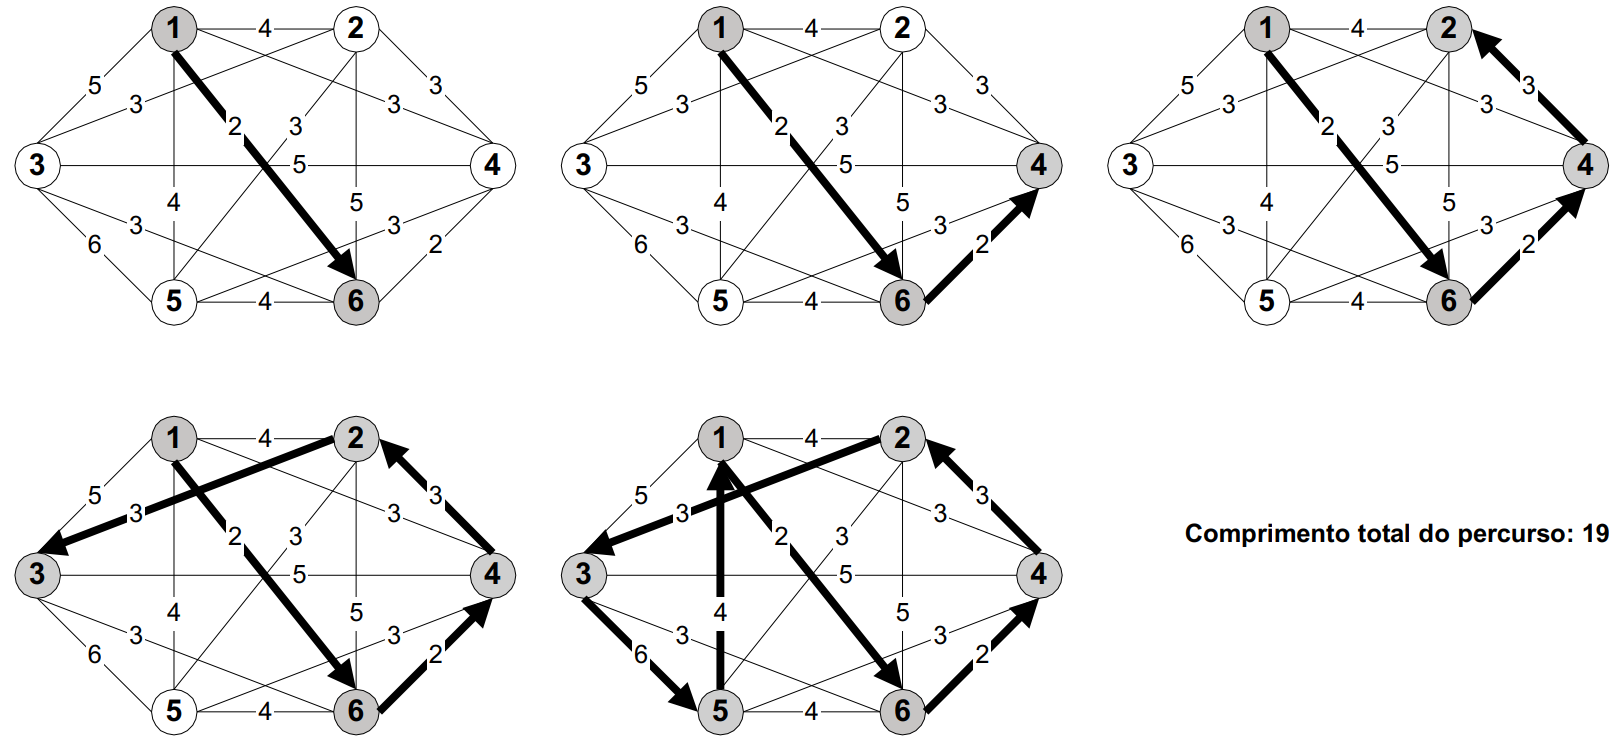
\includegraphics[width=1\textwidth]{vizinho.png}
	\caption{Execução da heurística de inserção do vizinho mais próximo}
	\label{fig:vizinho}
\end{figure*}

\subsubsection{Heurística melhorativa}
Dado uma solução inicial obtida pela heurística construtiva, a ideia é usar uma heurística melhorativa para fazer alterações na solução inicial buscando melhorar a qualidade.
Para isso foi usado a heurística melhorativa 2-opt.

O algoritmo 2-opt consiste em remover duas arestas não adjacentes da rota e reconectá-las usando duas outras arestas, de modo a reconstruir a rota e verificar se a houve melhora com a nova rota obtida. Repetindo esse processo para todos os pares de arestas possíveis, ao término, realizamos a melhor troca.

O algoritmo melhorativo 2-opt consiste em, dado uma rota.........

\textbf{falar codigo}

%imagem
\begin{figure*}[ht]
	\centering
	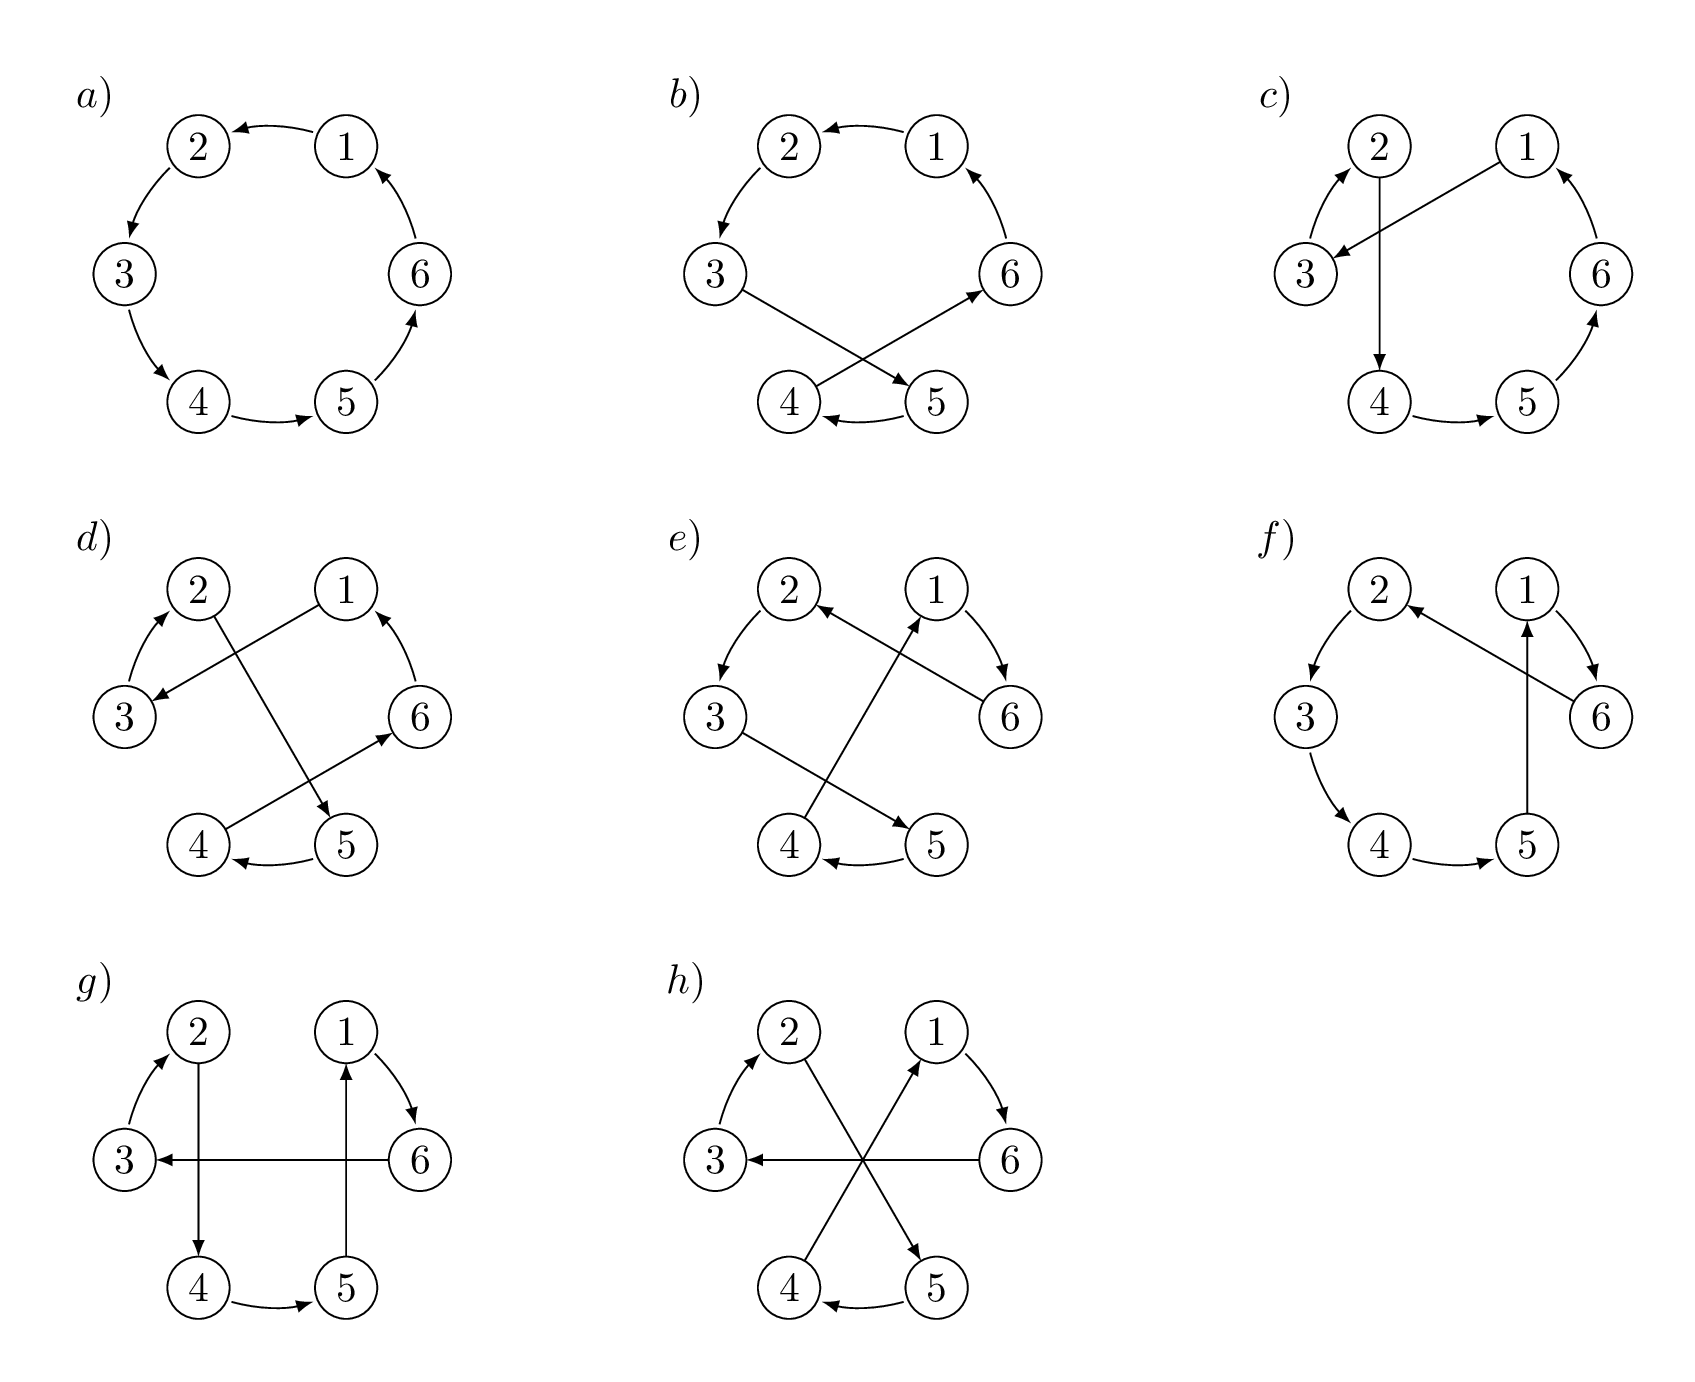
\includegraphics[width=1\textwidth]{2optnew.png}
	\caption{Execução da heurística 2-opt}
	\label{fig:2optnew}
\end{figure*}

\section{Base da dados}
Os algoritmos implementados foram executados usando as instâncias assimétricas do PCV da biblioteca TSPLIB.





\section{Como executar algoritmo} \label{sec:firstpage}

..........

\section{Dificuldades etc}

...........

\section{Resultados}

\section{Aplicações}

\begin{table}[!ht]
	\centering
	\caption{Valores de Similaridade por Usuário}
	\label{citacao6}
	\begin{tabular}{lcccc}
		\toprule
		\textbf{Instâncias}    & \textbf{Valor} \\ \midrule
		br17    & 1     \\ \midrule
		ftv33 & 1   \\ \midrule
		ftv35 & 1 \\ \midrule
		ftv38  & 1    \\ \midrule
		p43    & 1     \\ \midrule
		ftv44 & 1   \\ \midrule
		ftv47  & 1    \\ \midrule
		ry48p    & 1     \\ \midrule
		ft53 & 1   \\ \midrule
		ftv55  & 1    \\ \midrule
		ftv64    & 1     \\ \midrule
		ft70 & 1   \\ \midrule
		ftv70  & 1    \\ \midrule
		kro124p    & 1     \\ \midrule
		ftv170 & 1   \\ \midrule
		rbg323  & 1    \\ \midrule
		rbg358    & 1     \\ \midrule
		rbg403 & 1   \\ \midrule
		rbg443   & 1    \\ \bottomrule
	\end{tabular}
\end{table}

\section{Figures and Captions}\label{sec:figs}

Modo de citacao 1:
(Figure~\ref{fig:exampleFig1})\\
Modo de citacao 2:
 Figure~\ref{fig:exampleFig2}.
 
\begin{figure}[ht]
\centering
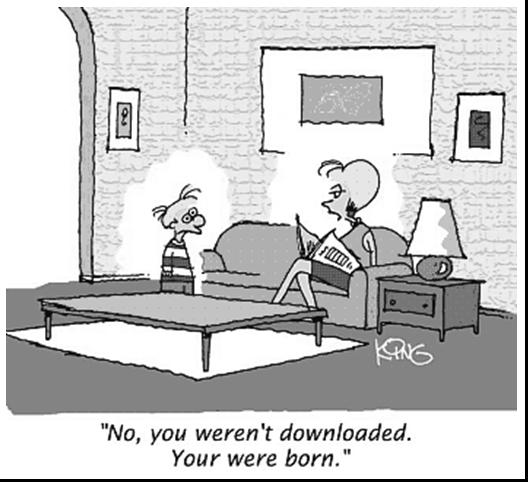
\includegraphics[width=.5\textwidth]{fig1.jpg}
\caption{A typical figure}
\label{fig:exampleFig1}
\end{figure}

\begin{figure}[ht]
\centering
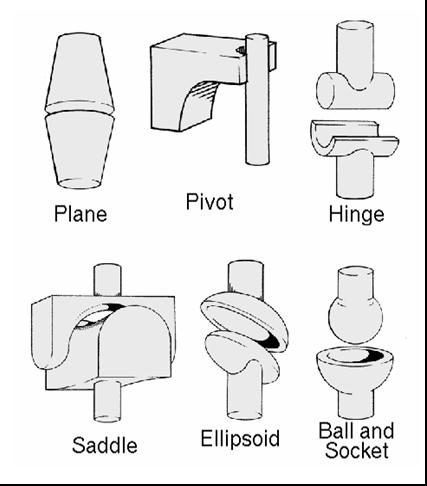
\includegraphics[width=.3\textwidth]{fig2.jpg}
\caption{This figure is an example of a figure caption taking more than one
  line and justified considering margins mentioned in Section~\ref{sec:figs}.}
\label{fig:exampleFig2}
\end{figure}

\begin{table}[ht]
\centering
\caption{Variables to be considered on the evaluation of interaction
  techniques}
\label{tab:exTable1}
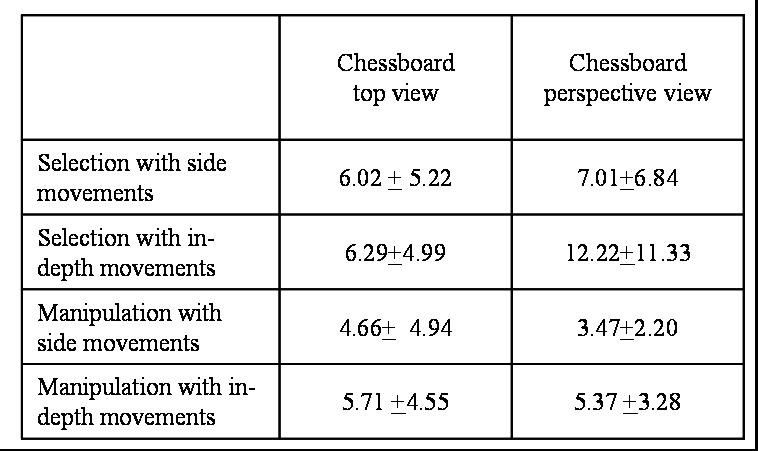
\includegraphics[width=.7\textwidth]{table.jpg}
\end{table}

%\begin{algorithm}
%	\caption{Vizinho mais próximo}
%	\begin{algorithmic}[1]
%		\Function{Absoluto}{x}
%		\If {$x < 0$}
%		\State \Return $-x$
%		\Else
%		\State \Return $x$
%		\EndIf
%		\EndFunction
%	\end{algorithmic}
%\end{algorithm}

\bibliographystyle{sbc}
\bibliography{sbc-template}
\end{document}
